\documentclass[border=10pt]{standalone}

\usepackage{tikz}
\usepackage{tikzsymbols}
\usetikzlibrary{calc,patterns,shapes.geometric}

\def\centerarc[#1](#2)(#3:#4:#5){\draw[#1] ($(#2)+({#5*cos(#3)},{#5*sin(#3)})$) arc (#3:#4:#5);}

\begin{document}
	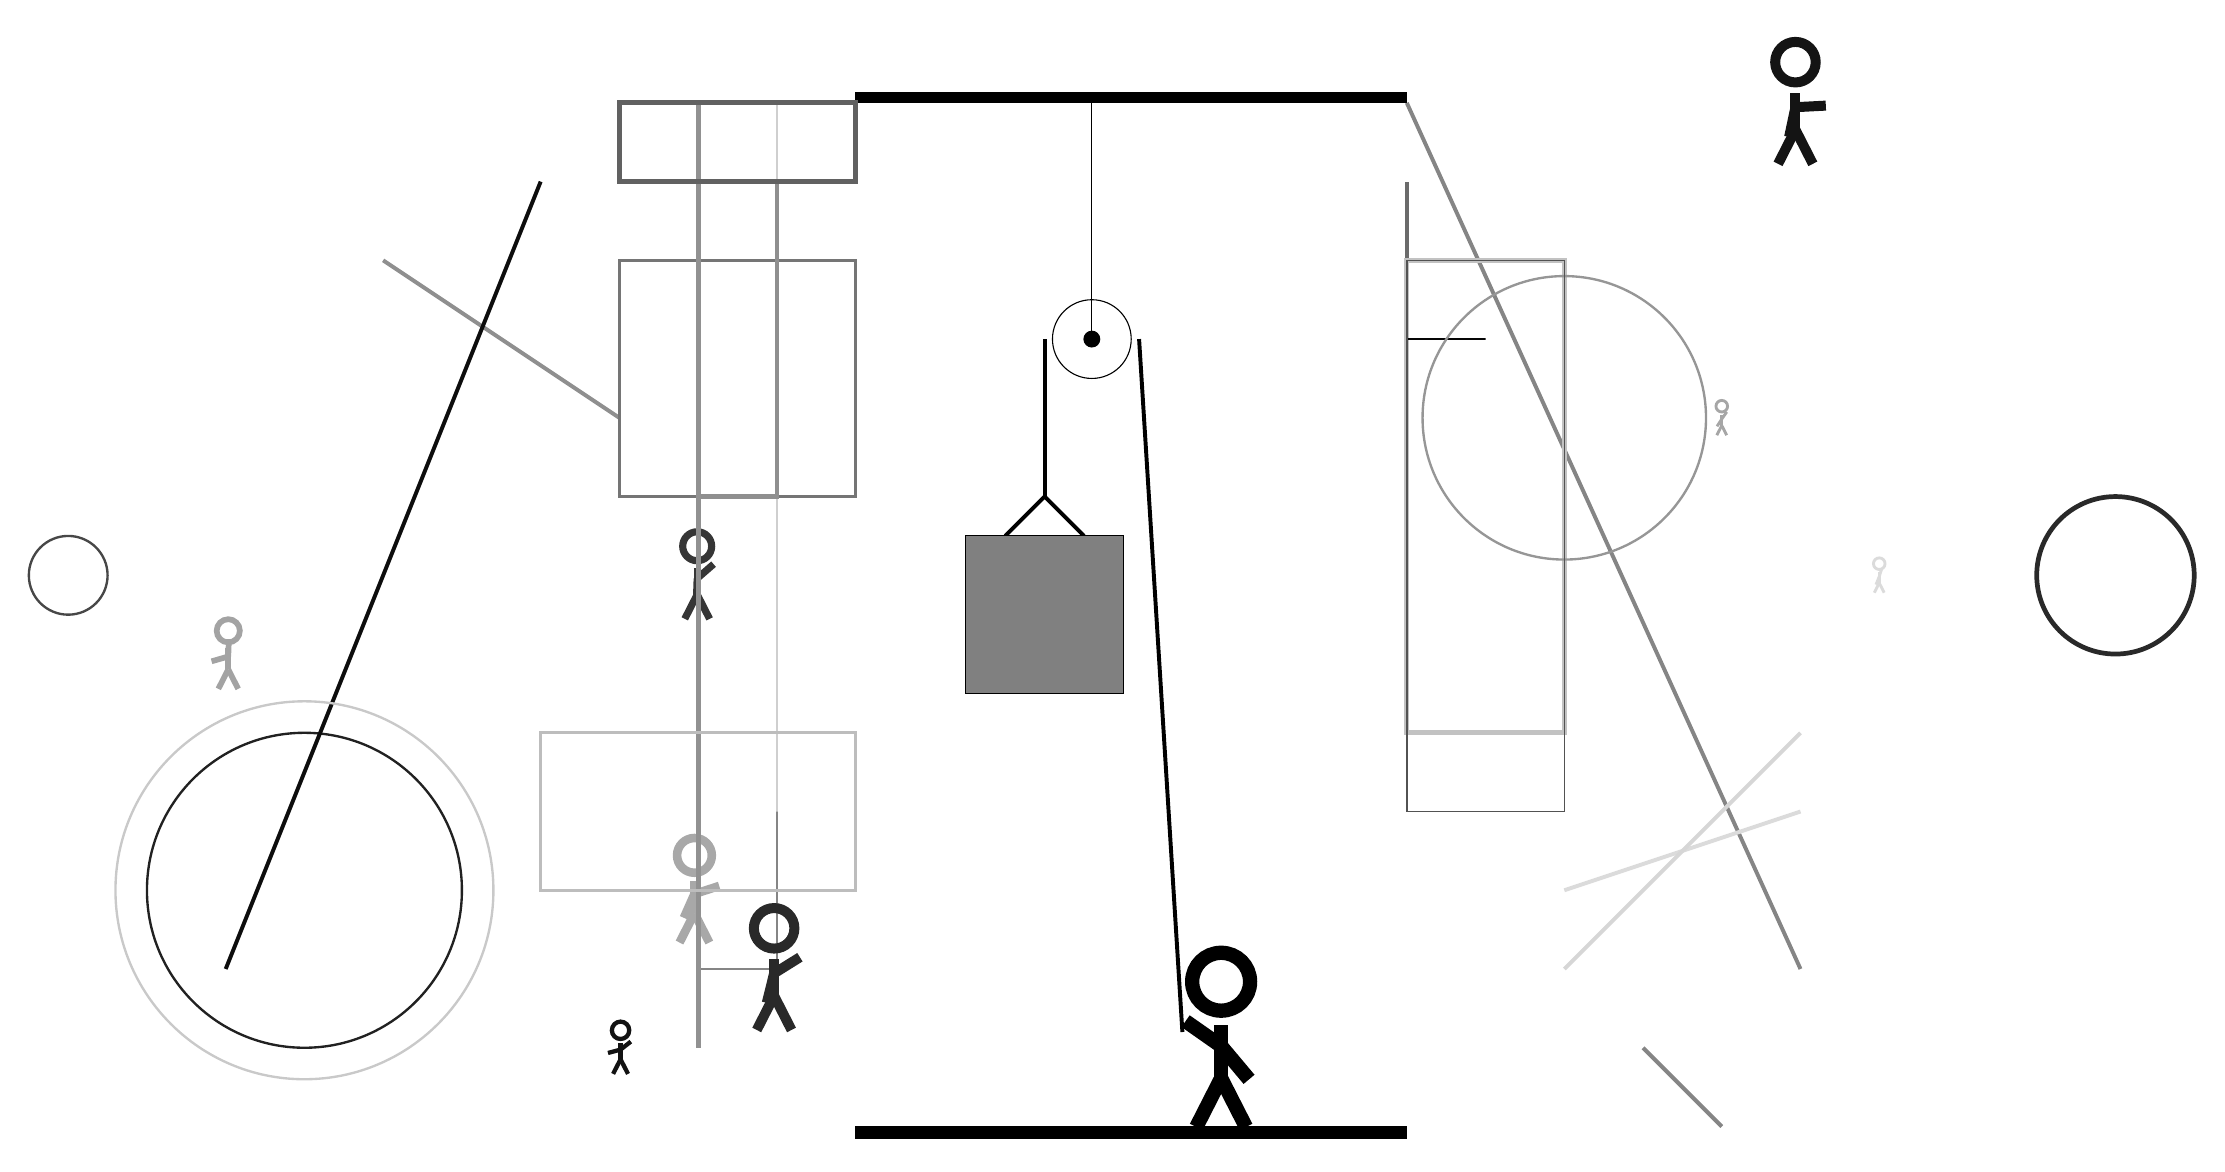
\begin{tikzpicture}
		%%%%% START %%%%%
		
		\draw[fill=black] (-2, 10) rectangle (5, 10.125);
		
		\draw (1, 7) circle (0.5);
		\draw[fill=black] (1, 7) circle (0.1);
		\draw (1, 10) -- (1, 7);
		
		\node[line width=0.6mm, color=black!35] at (9, 6) {\Strichmaxerl[2][57][55]};
		
		\draw[line width=0.2mm, color=black!48] (-4, -1) rectangle (-3, 5);
		\draw[line width=0.5mm, color=black!48](10, -1) -- (5, 10);
		\node[line width=0.2mm, color=black!36] at (-10, 3) {\Strichmaxerl[4][16][88]};
		
		\node[line width=0.4mm, color=black!79] at (-4, 4) {\Strichmaxerl[5][88][41]};
		
		\draw [line width=0.3mm, color=black!87](-9, 0) circle (2.0);
		\node[line width=0.6mm, color=black!34] at (-4, 0) {\Strichmaxerl[6][66][18]};
		\draw[line width=0.5mm, color=black!44](-5, 6) -- (-8, 8);
		\node[line width=0.5mm, color=black!14] at (11, 4) {\Strichmaxerl[2][68][72]};
		\draw [line width=0.6mm, color=black!84](14, 4) circle (1.0);
		\node[line width=0.3mm, color=black!84] at (-3, -1) {\Strichmaxerl[7][76][32]};
		\draw[line width=0.2mm, color=black!19] (-3, 1) rectangle (-3, 10);
		\draw[line width=0.4mm, color=black!54] (-2, 8) rectangle (-5, 5);
		\draw [line width=0.3mm, color=black!72](-12, 4) circle (0.5);
		\draw[line width=0.5mm, color=black!14](10, 1) -- (7, 0);
		\draw[line width=0.5mm, color=black!58](5, 2) -- (5, 9);
		\draw[line width=0.5mm, color=black!95](-6, 9) -- (-10, -1);
		\draw[line width=0.6mm, color=black!24] (5, 2) rectangle (7, 8);
		\draw[line width=0.5mm, color=black!38] (-3, 10) rectangle (-5, 10);
		
		\draw[line width=0.6mm, color=black!44] (-3, 9) rectangle (-4, 5);
		\node[line width=0.6mm, color=black!92] at (10, 10) {\Strichmaxerl[7][78][3]};
		
		\draw[line width=0.2mm, color=black!98] (6, 7) rectangle (5, 7);
		\draw[line width=0.6mm, color=black!43] (-4, -2) rectangle (-4, 10);
		\draw[line width=0.5mm, color=black!16](7, -1) -- (10, 2);
		\draw[line width=0.5mm, color=black!48](8, -2) -- (9, -3);
		
		\draw [line width=0.3mm, color=black!21](-9, 0) circle (2.4);
		\draw[line width=0.6mm, color=black!62] (-2, 9) rectangle (-5, 10);
		\draw[line width=0.4mm, color=black!26] (-2, 0) rectangle (-6, 2);
		\node[line width=0.2mm, color=black!93] at (-5, -2) {\Strichmaxerl[3][15][38]};
		\draw [line width=0.3mm, color=black!41](7, 6) circle (1.8);
		\draw[line width=0.2mm, color=black!68] (5, 8) rectangle (7, 1);
		
		\draw[line width=0.5mm] (-0.1, 4.5) -- (0.4, 5.0) -- (0.9, 4.5);
		\draw[fill=black!50] (-0.6, 4.5) rectangle (1.4, 2.5);
		
		\draw[line width=0.5mm] (0.4, 7) -- (0.4, 5.0);
		\centerarc[line width=0.5mm](1, 7)(0:180:0.6);
		\draw[line width=0.5mm](1.6, 7) -- (2.15, -1.8);
		
		\node at (2.6, -1.9) {\Strichmaxerl[10][-35][-50]};
		
		\draw[fill=black] (-2, -3) rectangle (5, -3.15);
		
		%%%%% END %%%%%
	\end{tikzpicture}
\end{document}